
\documentclass[fleqn,addpoints]{exam}

\usepackage{graphicx}
\usepackage{float}
\usepackage{amsmath}
\usepackage{cancel}
\usepackage{polynom}

\printanswers

\ifprintanswers
\usepackage{2in1, lscape}
\fi

\title{Math 115 Homework 1}
\date{September 21, 2010}

\begin{document}

% THIS HOMEWORK WAS TOO LONG

\maketitle

\ifprintanswers
\else
\section{Schedule}

Unfortunately, I have a conflict next week so we won't have class on 9/28.  We'll meet next on 10/5.

\fi

\section{From the Book}

Read pages 1-16.
 
\begin{itemize}
  \item p. 11: 13-23, 25-29, 31, 33, 37
  \item pp. 16-17: 14-20, 25-26, 28, 29, 31, 35, 36, 38
\end{itemize}

\ifprintanswers
\section{Page 11}
\begin{itemize}

\item[13]
\begin{align*}
  -2 < 3x - 2 < 5 \\
  0 < 3x  < 7 \\
  0 < x < \frac{7}{3} \\
\end{align*}

$x = \left(0, \dfrac{7}{3} \right)$

\item[14]
$-2 < 2x + 9 < 5 + x$

\begin{eqnarray*}
  -2 < 2x + 9 & and & 2x + 9 < 5 + x \\
  -11 < 2x    & and & 2x < -4 + x \\
  -\frac{11}{2} < x  & and & x < -4 \\
\end{eqnarray*}

$x = \left( -\dfrac{11}{2}, -4 \right)$

\item[15]
$(x+1)(x-2) \geq 0$ for $x = (-\infty, -1] \cup [2, \infty)$

\item[16]
\begin{align*}
  x^2 - 5x - 20 & \leq 4 \\
  x^2 - 5x - 24 & \leq 0 \\
  (x-8)(x+3) & \leq 0
\end{align*}

The interesting points are $x= \{-3, 8\}$ and the inequality is satisfied for: $x = (-3, 8)$.

\item[17]
$(x-2)(x+4)(x-3) \geq 0$ 

The interesting points are $x=\{2, -4, 3\}$ and the inequality is satisfied for: $x = [-4, 2] \cup [3, \infty)$

\item[18]
\begin{align*}
  x^3-6x^2+8x &< 0 \\
  x(x^2-6x+8) &< 0 \\
  x(x-4)(x-2) &< 0 \\
\end{align*}

The interesting points are $x=\{ 0, 2, 4\}$ and the inequality is satisfied for: $x = (-\infty, 0) \cup (2, 4)$.

\item[19]
\begin{align*}
  \frac{1}{x} & \leq 5 \\
  \frac{1}{x} - 5 & \leq 0 \\
  \frac{1}{x} - \frac{5x}{x} & \leq 0 \\
  \frac{1 - 5x}{x} & \leq 0 \\
\end{align*}

$x = (-\infty, 0) \cup \left[ \dfrac{1}{5}, \infty \right)$

\item[20]
\begin{align*}
  -2 & \leq \frac{1}{x} \\
  \frac{1}{x} + 2 & \geq 0\\
  \frac{1 + 2x}{x} & \geq 0\\
\end{align*}

$x = \left( -\infty, -\dfrac{1}{2} \right] \cup (0, \infty)$ 

\item[21]
\[
  \frac{3x+1}{x-1} \geq 0
\]

The interesting points are $x= \left \{ -\dfrac{1}{3}, 1 \right \}$ and the inequality is satisfied for: 
$x = \left(-\infty, -\dfrac{1}{3} \right] \cup (1, \infty)$.

\item[22]
\[
  \frac{(x-1)(x+2)} {x(x+1)} > 0
\]

The interesting points are $x= \{1, -2, -1, 0 \}$ and the inequality is satisfied for: 
$x = (-\infty, -2) \cup (-1, 0) \cup (1, \infty)$.

\item[23]
\begin{align*}
  \frac{2}{x-1} & \geq \frac{3}{x+2} \\
  \frac{2}{x-1} - \frac{3}{x+2} & \geq 0 \\
  \frac{7-x}{(x-1)(x+2)} & \geq 0 \\
\end{align*}

$x = (-\infty, -2) \cup (1, 7)$

\item[25]
\begin{align*}
  |5x| &= 2 \\
  5x = 2 & \text{ or } 5x = -2 \\
  x = \frac{2}{5} & \text{ or } x = -\frac{2}{5} \\
\end{align*}

$x = \left \{ -\dfrac{2}{5}, \dfrac{2}{5} \right \}$

\item[26]
\begin{align*}
  |2x+3| & = 1 \\
  2x+3 = 1 & \text{ or } 2x + 3 = -1 \\
  2x = -2 & \text{ or } 2x = -4 \\
  x = -1 & \text{ or } x = -2 \\
\end{align*}

$x = \{-2, -1\}$

\item[27]
\begin{align*}
  \left| \frac{x-1}{2x+3} \right| & = 2 \\
  \frac{x-1}{2x+3} = 2 & \text{ or } \frac{x-1}{2x+3} = -2 \\
  x-1 = 4x+6 & \text{ or } x-1 = -4x-6 \\
  -3x = 7 & \text{ or } 5x = -5 \\
  x = -\frac{7}{3} & \text{ or } x = -1 \\
\end{align*}

$x = \left\{ -\dfrac{7}{3}, -1 \right\}$

\item[28]
$|x-1| = |2x+1|$

There are four combinations, since either side can be either positive or negative:
\begin{align*}
  x-1 &= 2x + 1  \\
  x-1 &= -(2x+1) \\
  -(x-1) &= 2x+1 \\ 
  -(x-1) & = -(2x+1) \\
\end{align*}

There are some duplicates, so the only values that work are 
\[
  x=\{-2, 0\}
\]

\item[31]
\begin{align*}
  \frac{1}{|x+5|} &> 2 \\
  |x+5| &< \frac{1}{2} \\
\end{align*}

\begin{align*}
  -\frac{1}{2} < & x+5 < \frac{1}{2} \\
  -\frac{11}{2} < & x  < -\frac{9}{2}
\end{align*}

$x = \left( -\dfrac{11}{2}, -\dfrac{9}{2} \right)$

\item[33]
$|x^2-4| > 0$

\begin{align*}
  x^2-4 > 0 & \text{ or } -(x^2-4) > 0 \\
  x^2 > 4 & \text{ or } -x^2 + 4 > 0 \\
  x^2 > 4 & \text{ or } -x^2 > -4 \\
  x^2 > 4 & \text{ or } x^2 < 4 \\
\end{align*}

$x^2>4$ when $x > 2 \text{ or } x < -2$ and $x^2<4$ when $-2 < x < 2$.

So the only values which don't work are $2$ and $-2$ and the solution set is $(-\infty, -2) \cup (-2, 2) \cup (2, \infty)$.

Another way to look at this one is to notice that the absoulte value is always either zero or positive.  Saying that
an absolute value is greater than zero is the same as saying that it is not equal to zero.  

Therefore, this problem is equivalent to the simpler:
\begin{align*}
  x^2 - 4 & \neq 0 \\
  x^2 & \neq 4 \\
  x & \neq \pm 2 \\
\end{align*}

\item[37]

The height is greater than or equal to 64 when:
\begin{align*}
  -16t^2 + 48t + 128 &\geq 64 \\
  -16t^2 + 48t + 64 &\geq 0 \\
  t^2 -3t - 4 &\leq 0 \\
  (t-4)(t+1) &\leq 0 \\
\end{align*}

$t = [-1, 4]$

Negative numbers don't make sense as times, so the actual range is: $t = [0, 4]$ and the ball will be at least 64 feet
off the ground for the first 4 seconds.

\end{itemize}

\pagebreak

\section{Page 16-17}
\begin{itemize}

\item[14]
My graphing program doesn't understand ``and'', so I couldn't get it to graph the solution.

\item[15]

$4 \leq |x|$

\begin{figure}[H]
  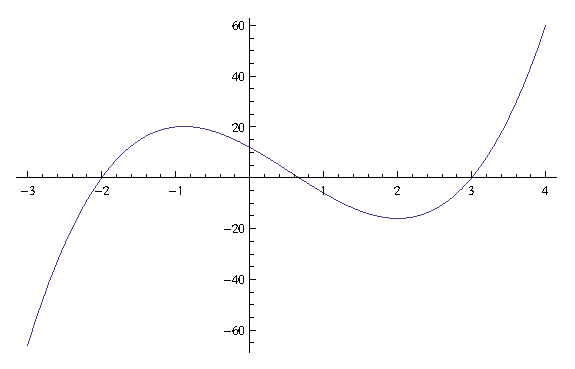
\includegraphics[width=12cm,height=7cm]{problem15}
\end{figure}

\pagebreak

\item[16]

$|y+1| < 2$

\begin{figure}[H]
  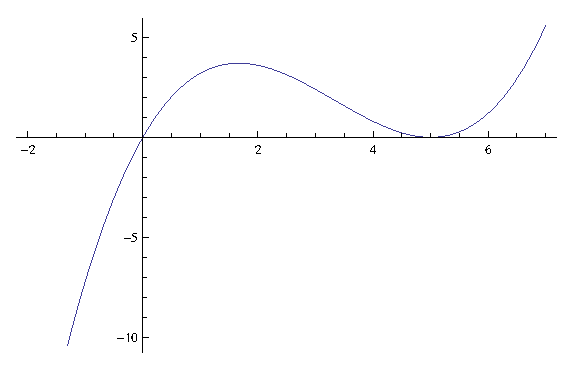
\includegraphics[width=12cm,height=7cm]{problem16}
\end{figure}

\item[17]
My graphing program doesn't understand ``and'', so I couldn't get it to graph the solution.

\item[18]
$|x| + |y| > 0$ is true for any $x$ or $y$ other than zero, so the graph is the entire x/y plane, excluding zero.

\item[19]
center: $(0, 0)$ and $r=1$

\begin{align*}
  (x-0)^2 + (y-0)^2 &= 1 \\
  x^2 + y^2 &= 1 \\
\end{align*}

\item[20]
center: $(-2, 3)$ and $r=2$

\[
  (x+2)^2 + (y-3)^2 = 4 \\
\]

\item[25]
$(x-2)^2 + (y-1)^2 = 9$

center: $(2, 1)$ and $r=3$

\item[26]
\begin{align*}
  x^2 - 4x + y^2 -2y &= 4 \\
  x^2 - 4x + 4 - 4 + y^2 -2y + 1 -1 &= 4 \\
  (x-2)^2 - 4 + (y-1)^2 -1 &= 4 \\
  (x-2)^2 + (y-1)^2 &= 9 \\
\end{align*}

center: $(2, 1)$ and $r=3$ (just like problem 25)

\item[28]
$\{(x, y) | x^2 + y^2 > 2\}$

\begin{figure}[H]
  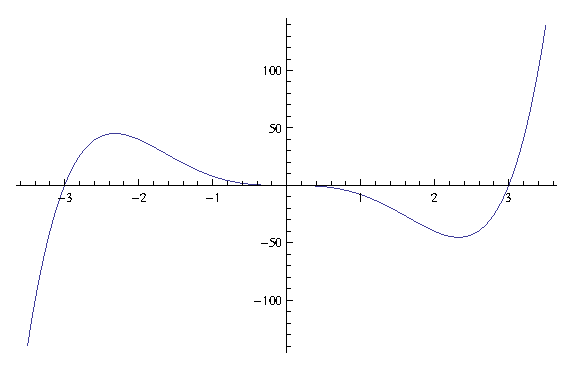
\includegraphics[width=12cm,height=7cm]{problem28}
\end{figure}

\item[29]
$\{(x, y) | 1 < x^2 + y^2 < 4\}$

I couldn't get my graphing program to do this one, but it would be a donut shape around the origin with an inner radius
of 1 and an outer radius of 2.

\item[31]
$P_1 = (-1, 4)$, $P_2 = (-3, -4)$, and $P_3 = (2, -1)$.

The distances are:
\begin{itemize}
  \item $d_{1,2} = \sqrt{(-1+3)^2 + (4+4)^2} = \sqrt{68}$
  \item $d_{1,3} = \sqrt{(-1-2)^2 + (4+1)^2} = \sqrt{34}$
  \item $d_{2,3} = \sqrt{(-3-2)^2 + (-4+1)^2} = \sqrt{34}$
\end{itemize}

Since $d_{1,3}^2 + d_{2,3}^2 = d_{1,2}^2$, the points form a right triangle with the right angle at $P_3$

% Another way to demonstrate that the points make a right triangle is with slopes.
% \begin{itemize}
%   \item $m_{1,3} = \dfrac{4+1}{-1-2} = -\dfrac{5}{3}$
%   \item $m_{2,3} = \dfrac{-4+1}{-3-2} = \dfrac{3}{5}$
% \end{itemize}

% Since $m_{1,3} \cdot m_{2,3} = -1$, the lines are perpendicular and meet at a right angle and so the triangle formed by
% the three points is a right triangle.

\item[35]
center: $(0, 0)$ passing through $(2, 3)$

The radius is: $r = \sqrt{(2 - 0)^2 + (3 - 0)^2} = \sqrt{13}$

So the equation is: $x^2+y^2 = 13$

\item[36]
center: $(1, 3)$ passing through $(-2, 4)$

The radius is: $r = \sqrt{(1+2)^2 + (3 - 4)^2} = \sqrt{10}$

So the equation is: $(x-1)^2+(y-3)^2 = 10$

\item[38]

If the point is on the y axis, its x coordinate is zero.

\begin{itemize}
  \item The distance from the first point is: $\sqrt{(-2)^2 + (y-1)^2}$
  \item The distance from the second point is: $\sqrt{(4)^2 + (y+3)^2}$
\end{itemize}

The distances need to be equal:
\begin{align*}
  \sqrt{(-2)^2 + (y-1)^2} &= \sqrt{(4)^2 + (y+3)^2} \\
  (-2)^2 + (y-1)^2 &= (4)^2 + (y+3)^2 \\
  4 + y^2 - 2y + 1 &= 16 + y^2 + 6y + 9 \\
  5  - 2y &= 25 + 6y  \\
    -8y &= 20  \\
    y &= -\frac{5}{2}  \\
\end{align*}

So the point is: $(0, -\dfrac{5}{2})$.

check:
  The distance from the first point is: 
\[
  \sqrt{(-2)^2 + \left( -\dfrac{5}{2} - 1 \right)^2} = \sqrt{4 + \dfrac{49}{4}} = \sqrt{\dfrac{65}{4}}
\]

The distance from the second point is: 
\[
  \sqrt{(4)^2 + \left( -\dfrac{5}{2}+3 \right)^2} = \sqrt{16 + \dfrac{1}{4}} = \sqrt{\dfrac{65}{4}}
\]

\end{itemize}

\fi

\section{Extra Credit}
\begin{questions}

\question
Ten people land on a deserted island. There they find lots of coconuts and a monkey. During their first day they gather
coconuts and put them all in a community pile. After working all day they decide to sleep and divide them into ten equal
piles the next morning.

That night one castaway wakes up hungry and decides to take his share early. After dividing up the coconuts he finds he
is one coconut short of ten equal piles. He also notices the monkey holding one more coconut. So he tries to take the
monkey's coconut to have a total evenly divisible by 10. However when he tries to take it the monkey conks him on the
head with it and kills him.

Later another castaway wakes up hungry and decides to take his share early. On the way to the coconuts he finds the body
of the first castaway, which pleases him because he will now be entitled to $1/9$ of the total pile. After dividing them
up into nine piles he is again one coconut short and tries to take the monkey's slightly bloodied coconut. The monkey
conks the second man on the head and kills him.

One by one each of the remaining castaways goes through the same process, until the tenth person to wake up gets the
entire pile for himself. What is the smallest number of possible coconuts in the pile, not counting the monkey's?

\begin{solution}

Since, counting the monkey's coconut, each person finds exactly the right number of coconuts for an even division with
the number of people still alive, the number of coconuts must be evenly divisible by 10, 9, 8, 7, 6, 5, 4, 3, and 2.  So
the smallest number of coconuts is the {\em Least Common Multiple} of these numbers which is:

\[
  2^3 \cdot 3^2 \cdot 5 \cdot 7 = 2,520
\]

The monkey's coconut is one of these, so the smallest number for the pile is 2,519.  

The last castaway gets 2,519 coconuts unless he gets greedy and tries to take the monkey's coconut, in
which case the monkey probably ends up with all the coconuts.

\end{solution}

\end{questions}

\ifprintanswers
\else
\vspace{1 in}

{\em I went to the woods because I wished to live deliberately, to front only the essential facts of life, and see if I
  could not learn what it had to teach, and not, when I came to die, discover that I had not yet lived.}

\vspace{.1 cm}
\hspace{1 cm} --Henry David Thoreau

\fi

\end{document}

